\documentclass{article}

\usepackage[margin=1in]{geometry}
\usepackage{graphicx}
\usepackage{amsmath}
\usepackage{booktabs}
\usepackage{float}
\usepackage[hidelinks]{hyperref}

\begin{document}

\title{Why the Radial Kernel Develops a Spike, and Why Different Kernels Can Perform Similarly}
\author{}
\date{2 April 2026}
\maketitle
\footnotesize
\setlength{\parindent}{0pt}

\section*{Question 1: Why does the learned radial kernel develop a spike?}

In \texttt{radial\_single\_kernel\_fi\_optimization.ipynb}, the radial kernel is parameterized as
\[
K(x,y)=\sum_{r=0}^{R} f_r\,B_r(x,y),
\]
where \(B_r\) is the binary mask of the integer-radius shell \(r\), and \(f_r\) is one learned coefficient per shell.

The spike is not an accident. It is a direct consequence of the optimization setup.

\subsection*{1. The seed kernel already contains the structure that later becomes the spike}
The radial model is not initialized from a flat or neutral profile. It starts from a circularized version of a previously learned kernel: the code first rotates the source kernel through many angles, averages those rotated copies to obtain a rotation-invariant circular kernel, and then converts that circular kernel into a shell-wise radial profile.

If the original source kernel has a stripe-like or band-like structure, that information does not disappear. After the circular averaging and radial projection, it becomes concentrated at particular radii. In radial coordinates, a preferred band in the original kernel is naturally converted into an elevated ring coefficient. That is why the spike should be understood first as an inherited feature of the rotation-invariant seed, not as something created entirely from scratch during later training.

\subsection*{2. The loss does not enforce a smooth or monotone radial profile strongly enough}
The original learned model uses
\[
\mathcal{L}
=
\mathcal{L}_{\mathrm{BCE}}
\;+\;
\lambda_{\mathrm{smooth}}\sum_r (f_r-f_{r-1})^2
\;+\;
\lambda_{\mathrm{anchor}}\sum_r (f_r-f_r^{\mathrm{seed}})^2
\;+\;
\lambda_{\mathrm{scale}}\left(\lVert f\rVert_2-\lVert f^{\mathrm{seed}}\rVert_2\right)^2.
\]

There is no hard monotonicity constraint, no explicit penalty against isolated peaks, and no requirement that the profile decays with radius. The smoothness term is weak compared with the classification objective, so once the initialization already contains a preferred radius, the optimizer is free to preserve or amplify that peak.

\subsection*{3. The scale penalty is applied to the coefficient vector, not to the 2D kernel energy}
This is the most important structural reason.

The regularizer constrains \(\lVert f\rVert_2\), but the actual 2D kernel energy depends on shell size:
\[
\lVert K\rVert_2^2
=
\sum_r |B_r|\, f_r^2,
\]
where \(|B_r|\) is the number of pixels in shell \(r\).

For the \(31\times31\) kernel used here, the first shell sizes are:
\[
1,\;8,\;16,\;20,\;24,\;40,\;36,\;48,\;56,\;56,\;68,\ldots
\]

So placing a large coefficient on radius \(r=5\) affects \(40\) pixels at once, while the same coefficient magnitude at the center affects only \(1\) pixel. In other words, the optimizer can create a strong ring-like detector at relatively low coefficient-norm cost. This makes shell spikes especially attractive.

\subsection*{4. Freezing outer radii concentrates the adjustment into a few inner bins}
The notebook sets
\[
\texttt{FREEZE\_OUTER\_RADII = True}
\]
and learns only radii \(0\) through \(20\), while keeping the outer tail fixed to the seed values. That means the optimizer has limited degrees of freedom. If it wants to improve classification, it must redistribute its learnable mass inside that restricted support. Concentrating mass into one or two shells is a natural outcome.

\subsection*{5. Training starts from that seed and refines it rather than removing it}
The saved seed radial coefficients are all near zero, while the learned unconstrained fit develops much larger values. For example, in the saved run:

\begin{itemize}
    \item seed coefficients are on the order of \(10^{-4}\) to \(10^{-3}\),
    \item the learned profile reaches about \(2.05\times10^{-2}\) at its strongest positive shell.
\end{itemize}

That jump shows that the optimizer is not inventing a totally unrelated profile. It is taking an already structured radial seed and amplifying one of its preferred radii because that improves discrimination.

\subsection*{Interpretation of the spike}
The spike should therefore be interpreted mainly as an \textbf{inherited and then amplified feature of the rotation-invariant seed kernel}, with the under-constrained optimization allowing that inherited peak to persist and sharpen. It is not strong evidence that the underlying lesion physics truly prefers a sharply spiky radial kernel.

In practical terms, the kernel ends up acting like a \textbf{ring detector}: if a patch contains contrast at roughly that radius, the response becomes strong, and the classifier benefits. The important point is that this preferred ring was already latent in the circularized seed and then strengthened during training.

\begin{figure}[H]
    \centering
    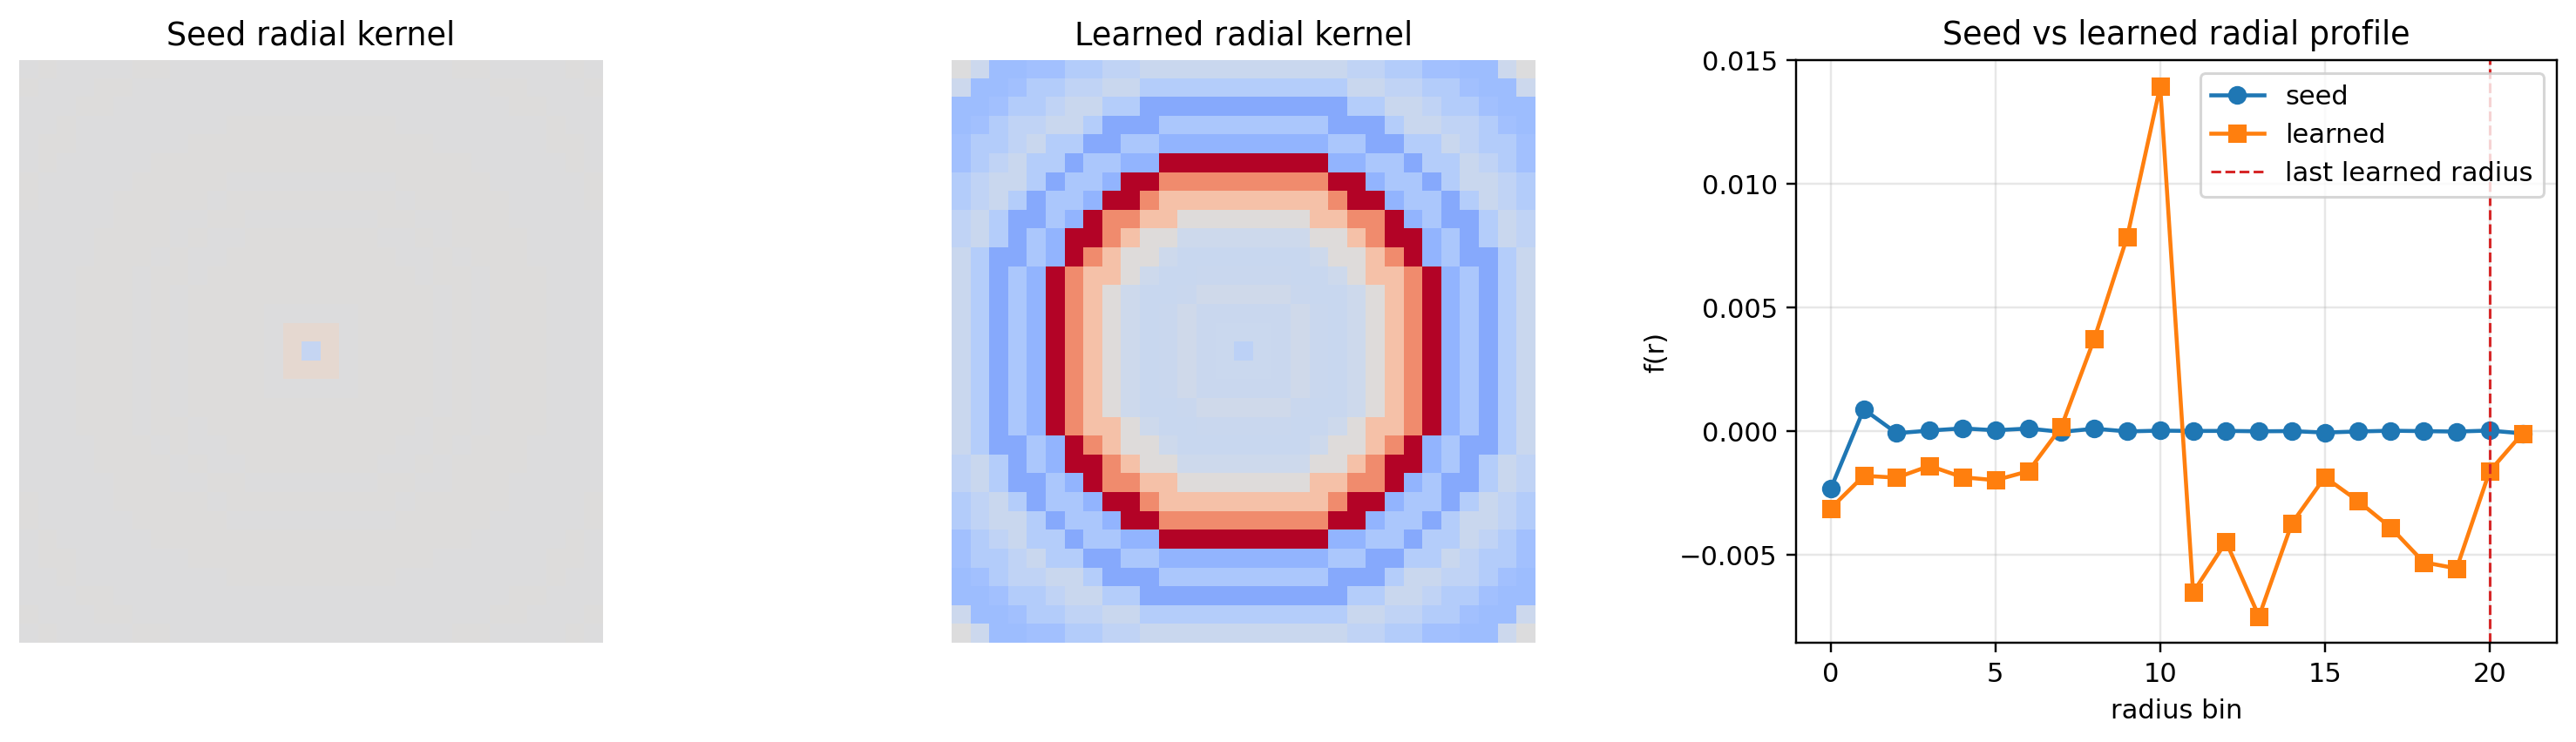
\includegraphics[width=0.98\textwidth]{figures/radial_single_kernel_current_summary.png}
    \caption{Current unconstrained radial fit. The sharp peak in the learned profile is the visible effect of the under-constrained \texttt{abs\_max} objective.}
\end{figure}

\subsection*{Why the constrained versions remove the spike}
The later notebook cells already confirm this diagnosis.

\begin{itemize}
    \item The monotone-decreasing version suppresses isolated spikes by construction.
    \item The signed compact version replaces \texttt{abs\_max} with a signed peak response, imposes a hard cutoff, and adds monotone/decay regularization.
\end{itemize}

These constrained versions produce kernels that are easier to interpret, even though their AUC is slightly lower than the unconstrained \texttt{abs\_max} fit. That tradeoff is exactly what one would expect: the original spike was helping classification in the narrow sense of the training objective, but it was not giving a unique or stable kernel shape.

\section*{Question 2: Why can very different kernels produce similarly good results?}

This also follows from the structure of the pipeline.

\subsection*{1. Many kernels generate highly correlated patch scores}
Your classifier usually does not consume the full response map. It consumes one or a few scalar summaries per patch, such as \texttt{abs\_max}, \texttt{mean\_abs}, or a small selected feature set. If two different kernels produce highly correlated scalar responses on the dataset, they are nearly interchangeable for classification.

This means the problem often has an \textbf{equivalence class of good kernels}: different filters may rank patches almost the same way, even if they look very different visually.

\subsection*{2. The dataset signal is likely coarse and low-dimensional}
The malignant-versus-healthy discrimination in these notebooks is not necessarily driven by one precise geometric template. It is more plausibly driven by broad image statistics:
\begin{itemize}
    \item local contrast,
    \item blob strength,
    \item edge density,
    \item texture roughness,
    \item lesion-versus-background intensity structure.
\end{itemize}

Many kernels can respond to those same coarse properties. A circular kernel, a square-like kernel, a triangular contrast kernel, and a radial ring kernel may all act as different probes of essentially the same underlying class signal.

\subsection*{3. Max-like response summaries erase shape information}
When the feature is based on a maximum absolute response, the detailed geometry of the kernel matters much less. The pipeline keeps only the strongest response magnitude, not where it occurred or what the full spatial response looked like.

As a result, very different kernels can collapse to similar one-dimensional features:
\[
\text{patch} \longmapsto \max |K * x|.
\]

Once the feature map is reduced to that scalar, many distinct kernels become behaviorally similar.

\subsection*{4. The classifier only needs a monotone separation, not a unique kernel}
The logistic calibration head does not require the feature to be physically meaningful. It only requires that positive and negative patches become more separable after a monotone transformation. If several kernels produce features with similar class ordering, then they will all produce similar AUC and similar accuracy after calibration.

\subsection*{5. Kernel search is often non-identifiable}
There is no guarantee of a unique optimum. Different kernels can compensate for one another through:
\begin{itemize}
    \item scaling,
    \item sign changes when absolute responses are used,
    \item support-width changes,
    \item different spatial shapes that still target the same lesion statistics.
\end{itemize}

This is why one can observe very different learned kernels with similar validation and test performance. The optimization is selecting one good representative from a large family of nearly equivalent solutions.

\section*{Main Conclusion}

The spike in the unconstrained radial kernel is mainly caused by the combination of:
\begin{itemize}
    \item \texttt{abs\_max} response aggregation,
    \item weak smoothness-only regularization,
    \item frozen outer radii,
    \item and a scale penalty on \(\lVert f\rVert\) rather than on the true 2D kernel norm.
\end{itemize}

So the spike is best understood as a \textbf{shortcut found by the optimizer}, not as a uniquely meaningful physical kernel shape.

The broader reason different kernels can all work well is that the classification pipeline only needs a small number of scalar patch features, and many visually different kernels produce very similar feature orderings on the data. In that regime, kernel appearance is not the same thing as kernel function. Several different kernels can therefore achieve similar AUC and accuracy because they are all measuring roughly the same discriminative image statistics.

\section*{Triangular and Square Notebook Comparison}

I also compared this with the notebook \texttt{kernel\_model\_triangular\_square\_short.ipynb}, which trains only two geometric kernel families: \texttt{triangular} and \texttt{square}. That notebook used the shape-sensitive setting with signed responses and patch standardization, and saved its results under:
\[
\texttt{results/triangular\_square\_shape\_sensitive/exp\_001}.
\]

\subsection*{Measured results}
The saved geometric-model runs report:
\begin{itemize}
    \item internal train-split validation: AUC \textbf{0.7610}, ACC \textbf{0.6915},
    \item held-out validation split: AUC \textbf{0.7407}, ACC \textbf{0.6631},
    \item held-out test split: AUC \textbf{0.8109}, ACC \textbf{0.7358}.
\end{itemize}

For the square-only variant, the saved run reports:
\begin{itemize}
    \item internal train-split validation: AUC \textbf{0.7584}, ACC \textbf{0.6890},
    \item held-out validation split: AUC \textbf{0.7399}, ACC \textbf{0.6631},
    \item held-out test split: AUC \textbf{0.7995}, ACC \textbf{0.7353}.
\end{itemize}

By comparison, the circularly symmetric radial approach performed better:
\begin{itemize}
    \item unconstrained radial/circular kernel: test AUC \textbf{0.9289}, test ACC \textbf{0.8684},
    \item signed compact radial/circular kernel: test AUC \textbf{0.8808}, test ACC \textbf{0.8011}.
\end{itemize}

So among the approaches compared here, the \textbf{circular (radial) kernel family is the strongest overall classification approach}. It gives the best quantitative results, and it remains competitive even after adding stronger interpretability constraints. The square-only model is slightly weaker than the mixed geometric model, which suggests that adding triangles helps a little, but not enough to close the gap to the radial approach.

\subsection*{Heatmap comparison}
The mixed triangular/square heatmap on \texttt{IMG015} is much more diffuse than the radial/circular one. It activates broad breast boundaries and widespread texture, rather than concentrating cleanly on the suspicious region. In particular, its reported mean probability is very high (\texttt{0.486}), which indicates that the model is assigning elevated scores across large parts of the breast instead of isolating the lesion.

The square-only model behaves almost the same way. Its \texttt{IMG015} heatmap has mean probability \texttt{0.497}, again indicating broad activation over the breast outline and internal texture rather than tight lesion localization. This qualitative similarity is consistent with the very similar test metrics of the square-only and mixed geometric runs.

The radial/circular heatmap, in contrast, is much more selective. Its energy is concentrated around the suspicious mass and nearby radiating structures, while the background remains mostly suppressed. That matches both the stronger test metrics and the visual impression that the circular model is detecting lesion-centered morphology more effectively.

\begin{figure}[H]
    \centering
    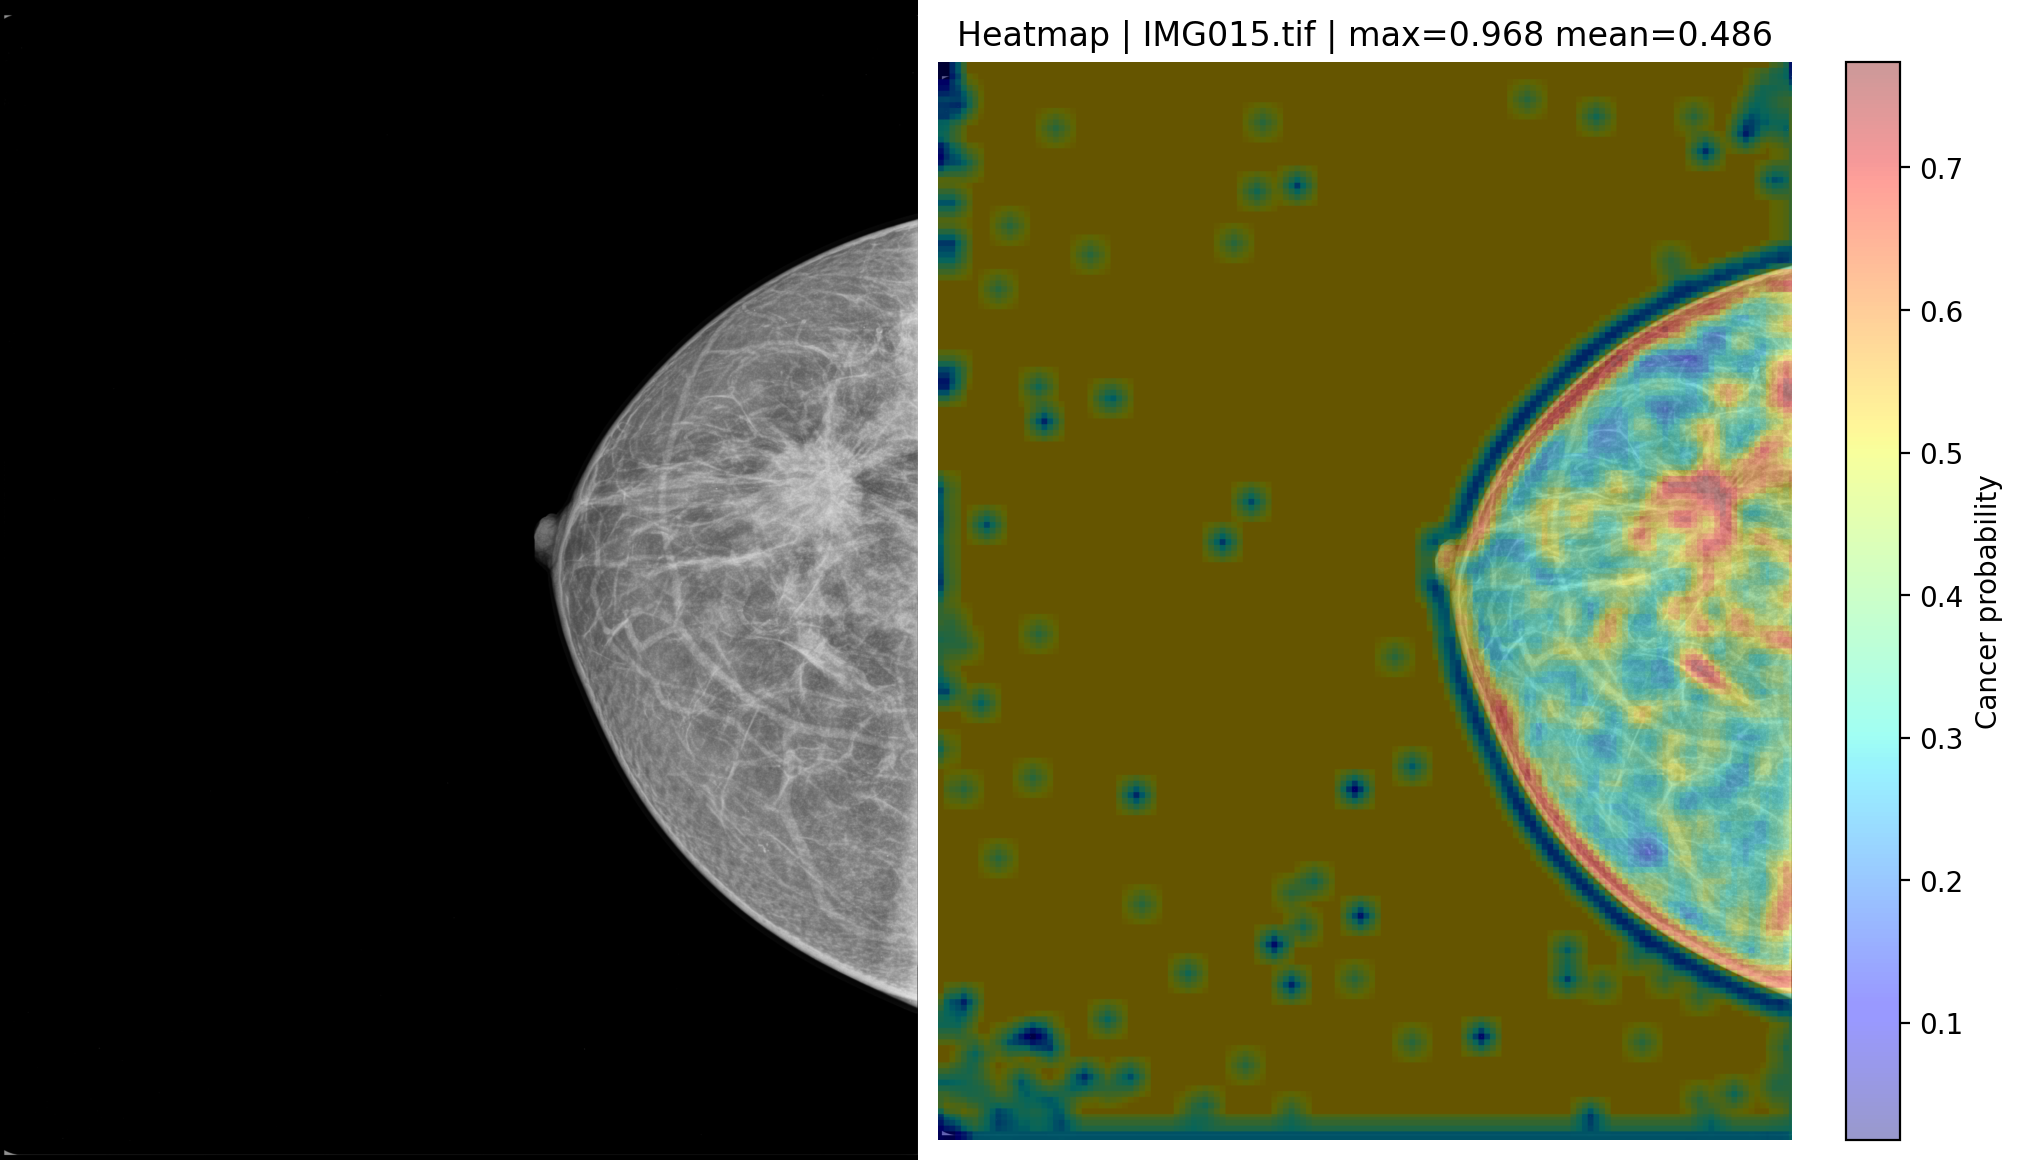
\includegraphics[width=0.49\textwidth]{../results/triangular_square_shape_sensitive/exp_001/heatmaps_pairs/IMG015_pair.png}
    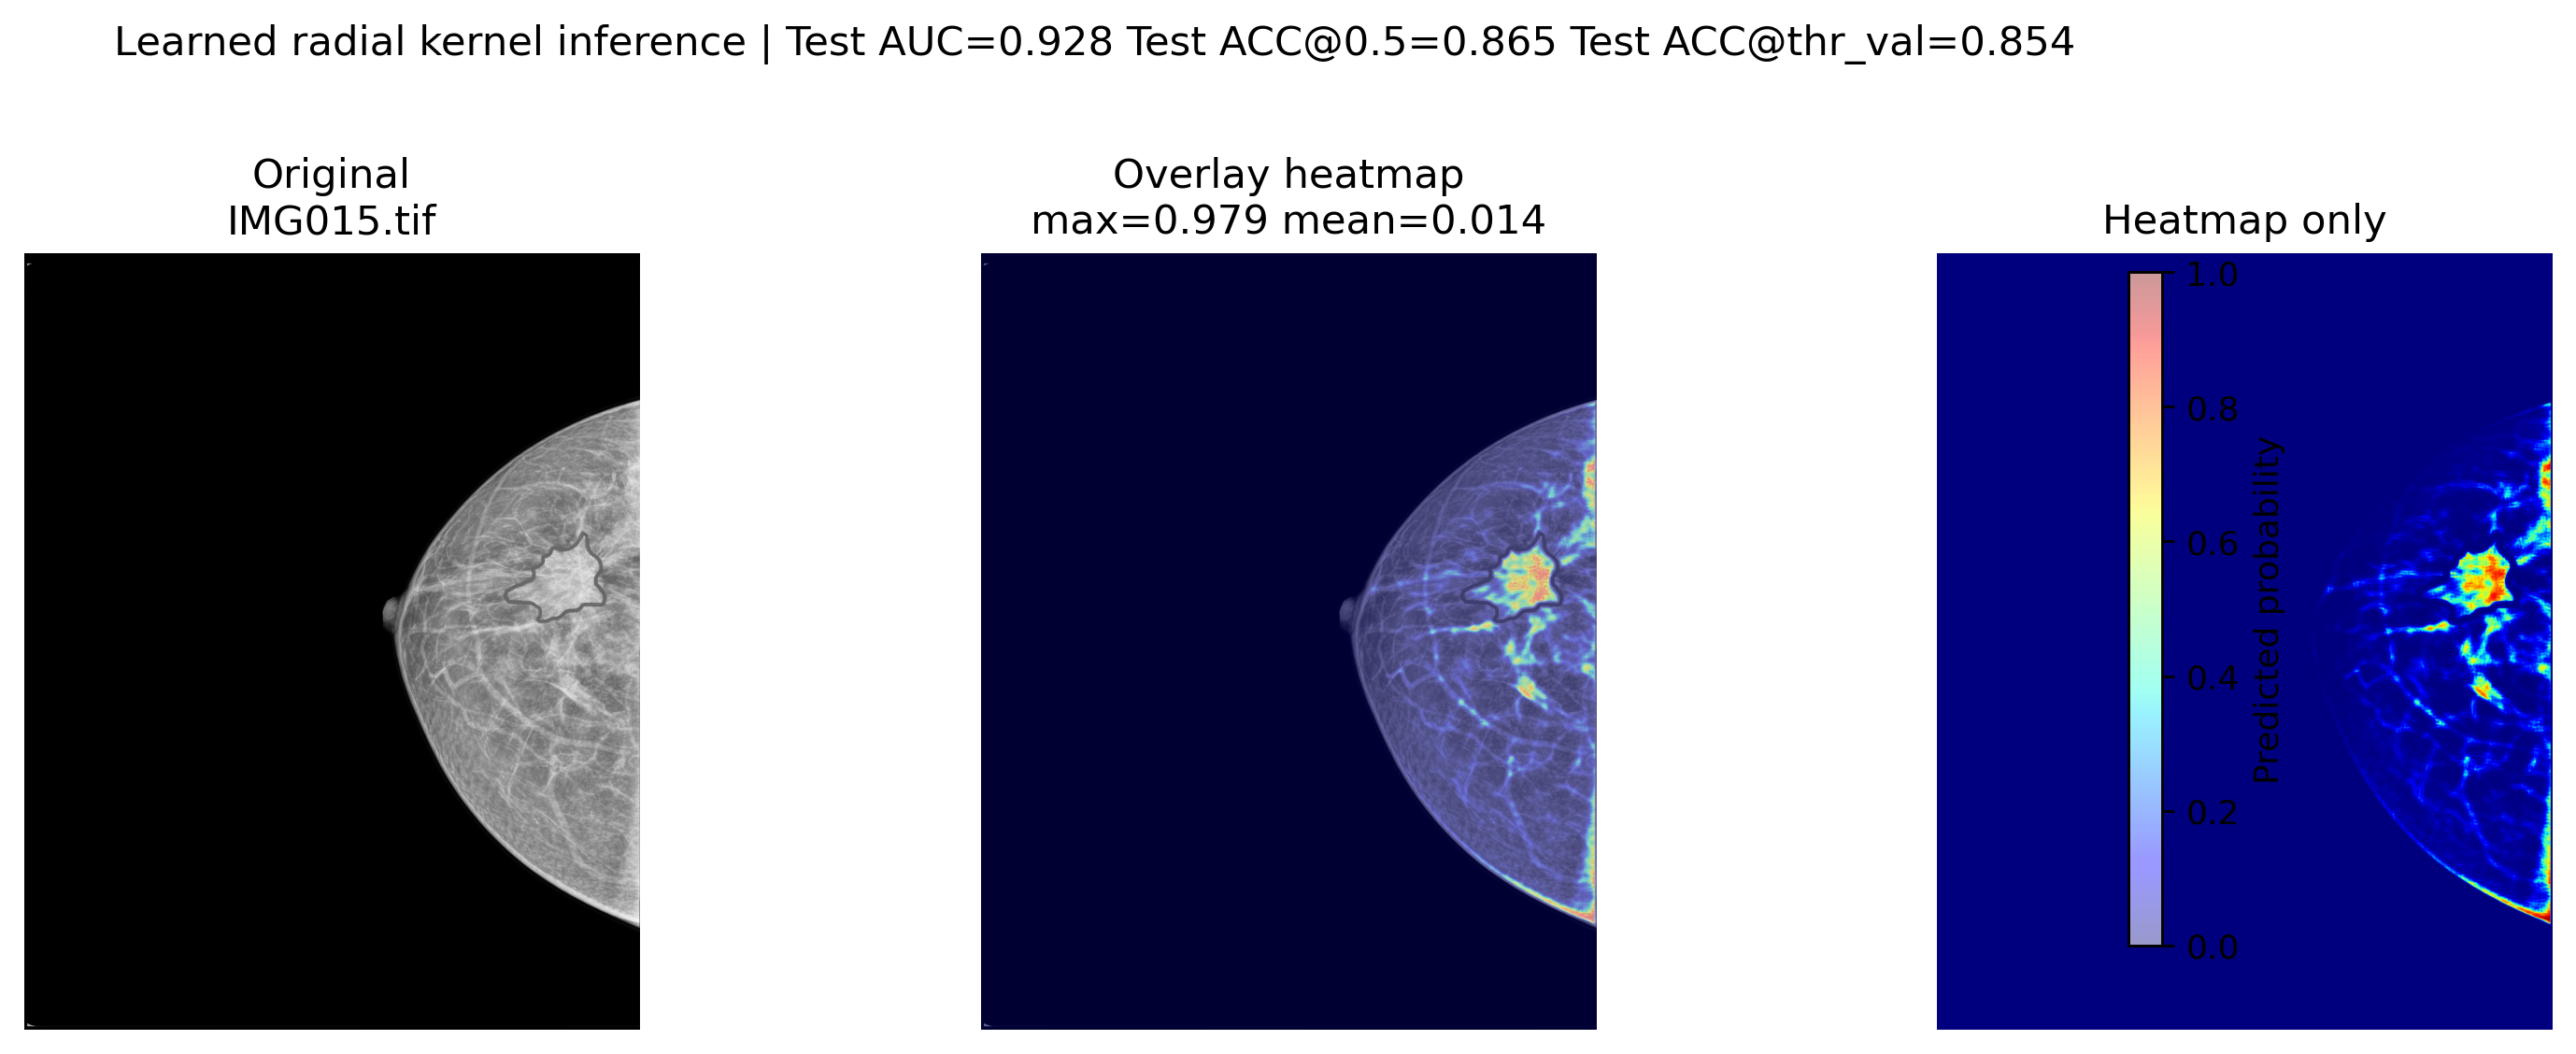
\includegraphics[width=0.49\textwidth]{figures/radial_single_kernel_heatmap.png}
    \caption{Left: triangular/square heatmap from \texttt{kernel\_model\_triangular\_square\_short.ipynb}. Right: learned radial/circular kernel heatmap. The geometric-kernel model spreads probability broadly over boundaries and texture, while the circular model is more localized and also achieves better test AUC and accuracy.}
\end{figure}

\subsection*{Interpretation}
This result makes sense for this cancer classification task. Many malignant regions in these mammograms are approximately blob-like or mass-like, with local structure that is better matched by circularly symmetric receptive fields than by hard-edged triangles or squares. The radial kernel is therefore a better inductive bias: it matches the morphology of the target structures more naturally, gives better patch discrimination, and produces more meaningful heatmaps.

\section*{Practical Implication}

If the goal is \textbf{best raw classification score}, the unconstrained kernel may remain attractive.

If the goal is \textbf{interpretable kernel shape and more trustworthy heatmaps}, then the constrained signed or monotone variants are the better direction, because they reduce the identifiability problem that creates the spike in the first place.

\end{document}
